\documentclass{amsart}
\usepackage{graphicx}
\graphicspath{{./}}
\usepackage{hyperref}
\usepackage{csvsimple}
\usepackage{longtable}
\usepackage{lscape}
\usepackage{epigraph}
\title{Ethnicity Effects on Confidence on Press}
\author{Zulfikar Moinuddin Ahmed}
\date{\today}
\begin{document}
\maketitle

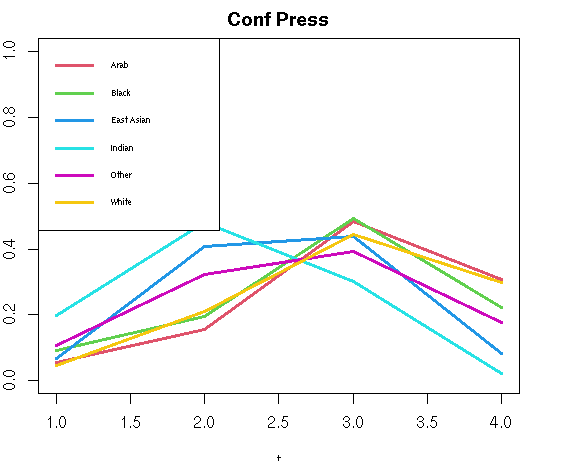
\includegraphics[scale=0.8]{cfpress_raw.png}

After fitting GHD we have the following.

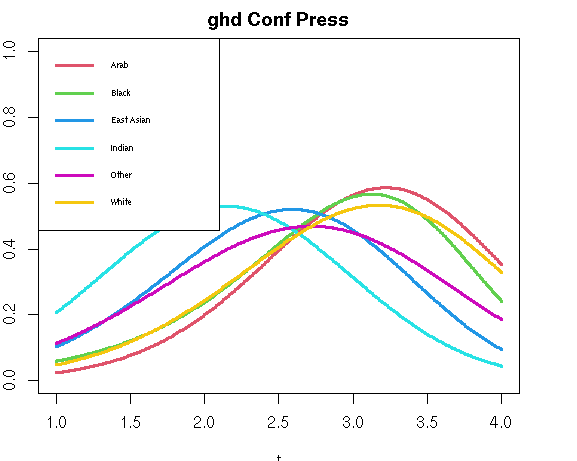
\includegraphics[scale=0.8]{cfpress_fitted.png}

Now visually, we can see that Whites, Blacks, and Arabs are very close together.

We can see Indians and East Asians are closer with higher confidence in Press, and "Other" are somewhere in between.

Let us now consider whether these visual features are detectable in the GHD parameter estimates.

% latex table generated in R 4.0.3 by xtable 1.8-4 package
% Mon May 17 23:50:42 2021
\begin{table}[ht]
\centering
\begin{tabular}{rlrrrrr}
  \hline
 & eth & lambda & mu & sigma & gamma & alpha.bar \\ 
  \hline
1 & Arab & -22.70 & 4.32 & 0.78 & -1.17 & 12.32 \\ 
  2 & Black & -4.34 & 3.80 & 0.78 & -0.94 & 2.12 \\ 
  3 & East Asian & -219.88 & 15.67 & 0.00 & -13.18 & 125.14 \\ 
  4 & Indian & -841.78 & 3.35 & 0.83 & -1.20 & 500.00 \\ 
  5 & Other & -517.38 & 26.75 & 0.02 & -24.10 & 318.88 \\ 
  6 & White & -129.95 & 14.12 & 0.00 & -11.08 & 81.61 \\ 
   \hline
\end{tabular}
\end{table}

We can see here something new, which is that the ordering of ethnicities by $\bar{\alpha}$ would give us our observed clustering.

\section{Code}

\begin{verbatim}
g<-function( theta ){
  lambda<-theta[1]
  mu <- theta[2]
  sigma <- theta[3]
  gamma <- theta[4]
  alpha.bar <- theta[5]
  out <- ghyp( lambda=lambda,mu=mu,sigma=sigma,
               gamma=gamma,alpha.bar=alpha.bar)
  out
}

fit_ghd_shape<-function( t, z0 ){
  delta <- t[2]-t[1]
  eps<-1e-6
  z<-cubicspline(1:length(z0),z0,xi=t)
  z[z<eps]<-eps
  z<-z/(sum(z[t>0.5 & t<4.5])*delta)
  y<-z
  objective<-function( theta ){
    yp <- dghyp( t, object=g(theta))
    out<-sum( delta*(y[t>0.9 & t<4.3]- yp[t>0.9 & t < 4.3])^2)
    if (is.na(out)){
      print(theta)
      print(yp)    
    }
    out
  }
  theta0 <-c(-3.0,3.5,1.1,0.0,1.0)
  lower0<-c(-1000,0,0.001,-Inf,0)
  upper0<-c(Inf,100,Inf,Inf,500)
  res<-optim( theta0, fn=objective,
              lower=lower0,
              upper=upper0,
              method="L-BFGS-B",control=list(trace=1,maxit=5000))
  
  yp<-dghyp( t, object=g(res$par))
  list(theta=res$par,t=t,x=z,y=yp)
}

fit_ghd_table<-function( A ){
  t<-seq(0,5,by=0.01)
  idx<-which(t>=1.0 & t<= 4.0)
  nrow.A <- dim(A)[1]
  A.interp<-matrix(0,nrow=nrow.A,ncol=length(idx) )
  A.fitted<-matrix(0,nrow=nrow.A,ncol=length(idx) )
  thetas<-data.frame()
  delta<-t[2]-t[1]
  for (k in 1:nrow.A){
    cur.fit<-fit_ghd_shape(t,A[k,])
    thetas<-rbind( thetas, c( row.names(A)[k], cur.fit$theta))
    A.interp[k,] <- nrm(cur.fit$x[idx])/delta
    A.fitted[k,] <- nrm(cur.fit$y[idx])/delta
  }
  names(thetas)<-c("eth",
                   "lambda", "mu", "sigma",
                   "gamma","alpha.bar")
  for (r in 2:6){
    thetas[,r]<-as.numeric(thetas[,r])
  }
  
  row.names(A.interp)<- row.names(A)
  row.names(A.fitted)<- row.names(A)
  
  list(theta=thetas, interp=A.interp, fitted=A.fitted, t=t[idx])
}

stack.plot<-function( A, title, position="topleft", t=NULL){
  if (is.null(t)){
    t<-1:dim(A)[2]
  }
  par(mar=c(3.5,2,2,3))
  q<-plot(t, A[1,], type='l',lwd=3,ylim=c(0,1.0), col=1+1, main=title)
  n<-dim(A)[1]
  for ( j in 2:n){
    lines(t,A[j,], lwd=3, col=j+1)
  }
  legend(position,legend=row.names(A),col=seq(2,1+n),lwd=3,
         cex=0.5)
  q
}

# Actual use here. 
# CfPress is row normalized
# table of eth, Q66

cfpress.out<-fit_ghd_table(CfPress)

stack.plot(cfpress.out$fitted,"ghd Conf Press",t=cfpress.out$t)
\end{verbatim}

\end{document}